\scanpage{120}
\mspage{111}
% archive sheet number: 120 (lower left)
% L1-4
Parmi les sommets internes, on distingue les sommets propres, ou \uline{sommets} \uline{redondants} ou ``sommets de morcellement'', et les sommets impropres, ou \uline{sommets} \uline{lacunaires}.

Dans la préfigure
\figure{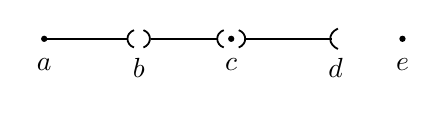
\begin{tikzpicture}[line width=.65pt]
\draw (0,0)--(1.05,0); \draw (1.35,0)--(2.2,0); \draw (2.55,0)--(3.65,0);
\fill (0,0) circle (.04); \fill (2.375,0) circle (.04); \fill (4.55,0) circle (.04);
\draw (1.14,.11) .. controls (1.03,.07) and (1.03,-.07) .. (1.14,-.11);
\draw (1.26,.11) .. controls (1.37,.07) and (1.37,-.07) .. (1.26,-.11);
\draw (2.28,.11) .. controls (2.17,.07) and (2.17,-.07) .. (2.28,-.11);
\draw (2.47,.11) .. controls (2.58,.07) and (2.58,-.07) .. (2.47,-.11);
\draw (3.73,.13) .. controls (3.60,.07) and (3.60,-.07) .. (3.73,-.13);
\node[below] at (0,-.12) {$a$}; \node[below] at (1.2,-.12) {$b$};
\node[below] at (2.375,-.12) {$c$}; \node[below] at (3.7,-.12) {$d$};
\node[below] at (4.55,-.12) {$e$};
\end{tikzpicture}}
il y a un sommet de chacun des cinq types combinatoires
\diagram{\(\begin{array}{ll}
\text{sommet isolé}&e\\
\text{sommet bord propre}&a\\
\text{\rule{2.4cm}{.3pt}\ impropre}&d\\
\text{sommet interne propre ou redondant}&c\\
\text{sommet interne impropre ou lacunaire}&b
\end{array}\)}

% L12-17
\deleted{\unsure{Pour que intervalles}}
Je préfère à présent appeler $S_{a,b}=S_{b,a}$ ou $S_{\{a,b\}}$ un intervalle (plutôt qu'un segment). Le \uline{segment} associé à l'intervalle est $\widetilde{S}_{a,b}=\{S_{ab},a,b\}$ --- c'est le \unsure{multistrate} complet associé à $S_{ab}$.

\deleted{\unsure{Si} $X\in\Phi_{\unsure{T_D|D}}$} On a posé
\[
\underbrace{\Phi_0\unsure{>|=}\Phi\cap\unsure{M|\mathcal{M}}_0=\Phi\cap\unsure{\mathcal{L}|L}}_{\substack{\text{ou ens. des sommets}\\\text{propres.}}},\quad\Phi_1=\Phi\cap M_1
\]
% L18-end: cancelled by long diagonal strokes.
\deleted{Pour les éléments de $\Phi_1$, ou \uline{intervalles de $\Phi$}, on distingue les intervalles de $\Phi$ tels que $\widetilde{X}\subset\Phi$ i.e. $\overline{X}\subset\Phi$ \inserted{i.e. $\unsure{\partial|\delta}X\subset\Phi_0$} (on peut les appeler \uline{fermés} \uline{dans} $\Phi$), \deleted{et} ceux pour lesquels $\partial X\cap\Phi_0=\{a\}$ (\uline{semi}-\uline{ouverts} \unsure{droits|droit}}
